
% Slideshow, written by Brent Baccala, for a summary lecture of calculus

\documentclass{beamer}
\usetheme{Madrid}

\title{History of Calculus}
\author{Brent Baccala}
\institute{\tt cosine@freesoft.org}
%% \date{February 8, 2023}

\setbeamertemplate{footline}{}
\beamertemplatenavigationsymbolsempty

\usepackage{amsmath}
\usepackage{tabularx}

\usepackage{breqn}

\usepackage{xcolor}
\usepackage{comment}
\usepackage{graphicx}

\usepackage{tabularx}

\usepackage{fancyvrb}

\usepackage{tikz}
\usetikzlibrary{positioning}
\usetikzlibrary{fit}
\usetikzlibrary{backgrounds}
\usetikzlibrary{angles,quotes,3d}
\usetikzlibrary{decorations.pathreplacing}
\usetikzlibrary{calc,intersections}
\usepackage{tikz-3dplot}

\usepackage{pgfplots}
\pgfplotsset{compat=1.16}

\usepackage{adjustbox}

\begin{document}


\begin{frame}
\titlepage
\begin{block}{Abstract}
A history of calculus
\end{block}
\end{frame}

\begin{frame}
\frametitle{Prototypical Calculus Problem}
\begin{center}
Find the area of a plane region

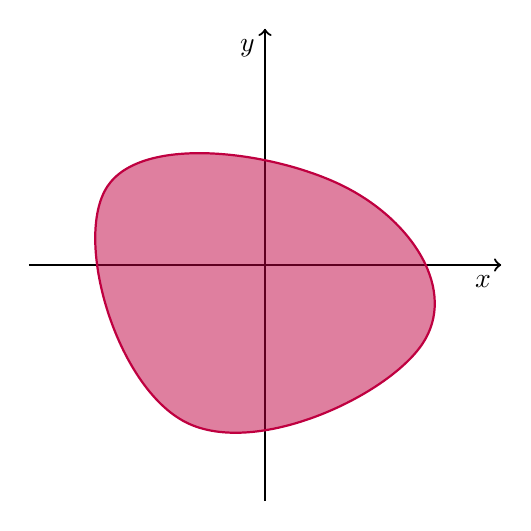
\begin{tikzpicture}[scale=1]

% Draw axes
\draw[thick,->] (-3,0) -- (3,0) node[anchor=north east]{$x$};
\draw[thick,->] (0,-3) -- (0,3) node[anchor=north east]{$y$};

% Draw shaded blob
\fill[purple, opacity=0.5] plot[smooth cycle, tension=0.8] coordinates {(-1,-2) (2,-1) (1,1) (-2,1)};
\draw[purple, thick] plot[smooth cycle, tension=0.8] coordinates {(-1,-2) (2,-1) (1,1) (-2,1)};

\end{tikzpicture}

\end{center}
\end{frame}

\begin{frame}
https://mathcs.clarku.edu/~djoyce/java/elements/bookXII/propXII2.html

Euclid 300 BC
Definition: $\pi = \frac{C}{D}$
Theorem: $A = \pi r^2$
C: circumference
D; diameter
A: area
r: radius

\begin{itemize}
\item An infinite series of {\it inscribed} polygons have area approaching a limit
\item An infinite series of {\it circumscribed} polygons have area approaching a limit
\item It's the same limit
\item Then the limit must be the area of the circle
\end{itemize}

\end{frame}

\begin{frame}

Archimedes c. 287 BC - c. 212 BC

Found the constant and proved the theorem $A=\pi r^2$

% This got GPT-4 close, then I polished it off:
%
% draw a new tikzpicture.  On the left I want a circle sliced up like a
% pie into eight equal slices.  On the right I want eight triangles of
% roughly the same size as the slices in the pie, lined up horizontally
% one right after the other.  Below the triangles draw a horizontal
% brace with "~c" below it.  To the right of the triangles draw a
% vertical brace with "~r" next to it.

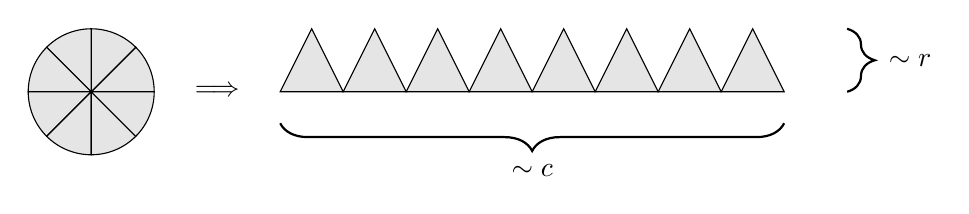
\begin{tikzpicture}[scale=0.8]

% Draw the pie
\foreach \i in {0,...,7}
{
  \draw[fill=gray!20] (0,0) -- (\i*45:1) arc (\i*45:\i*45+45:1) -- cycle;
}

% Draw the triangles
\foreach \j in {0,...,7}
{
  \draw[fill=gray!20, xshift=3cm] (\j,0) -- (\j+1,0) -- (\j+0.5,1) -- cycle;
}

\node at (2,0) {$\Longrightarrow$};

% Draw the braces
\draw[thick, decorate, decoration={brace, amplitude=10pt, mirror}, yshift=-0.5cm, xshift=3cm] (0,0) -- (8,0) node[midway, yshift=-0.6cm] {$\sim c$};
\draw[thick, decorate, decoration={brace, amplitude=10pt, mirror}, xshift=12cm] (0,0) -- (0,1) node[midway, xshift=0.8cm] {$\sim r$};

\end{tikzpicture}

\[ A \approx \frac{1}{2} c r = \pi r^2 \]
\end{frame}

\begin{frame}
Archimedes Method of Exhaustion

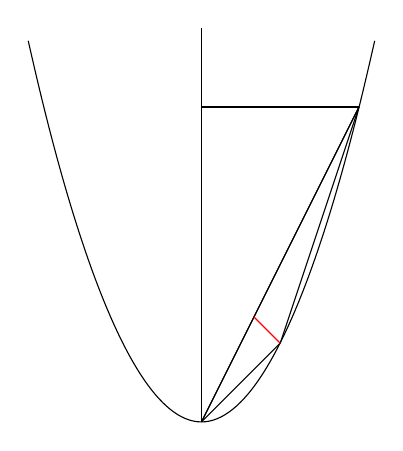
\begin{tikzpicture}

% Draw the parabola
%\draw[-] (-2,4) parabola bend (0,0) (2,4);
\draw[-] (-2.2,4.84) parabola bend (0,0) (2.2,4.84);

% y axis
\draw (0,0) -- (0,5);

\draw (0,4) -- (2,4);

\draw (0,0) -- (2,4);

\draw (0,0) -- (1,1);
\draw (1,1) -- (2,4);

% Define the points for line A
\coordinate (A) at (0,0);
\coordinate (B) at (2,4);

% Define the midpoint of line A
\coordinate (M) at ($(A)!0.5!(B)$);

% Define the point (1,1)
\coordinate (P) at (1,1);

\draw[name path=line A] (A) -- (B);

% Draw the line through (1,1) perpendicular to line A
\path[name path=line P] (P) -- ($(P)!2cm!-90:(A)$);

% Calculate intersection of lines
\path[name intersections={of=line A and line P, by=I}];

% Draw the line from (1,1) to the intersection point
\draw[red] (P) -- (I);

\end{tikzpicture}

Area of parabola = 4/3 area of inscribed triangle

\end{frame}

\begin{frame}
\frametitle{Method of Indivisibles}
Cavalieri 1598-1647

add a parabola

\tdplotsetmaincoords{70}{110}

\begin{tikzpicture}[tdplot_main_coords, line join = round, line cap = round]

% Define the main coordinates
\coordinate (O) at (0,0,0);
\coordinate (A) at (2,2,0);
\coordinate (B) at (-2,2,0);
\coordinate (C) at (-2,-2,0);
\coordinate (D) at (2,-2,0);
\coordinate (E) at (0,0,3);

% Draw the pyramid
\draw[fill=blue!20] (A) -- (B) -- (C) -- (D) -- cycle;
\draw (A) -- (E);
\draw (B) -- (E);
\draw (C) -- (E);
\draw (D) -- (E);

% Draw the slices
\draw[dashed] (1,1,1) -- (-1,1,1) -- (-1,-1,1) -- (1,-1,1) -- cycle;
\draw[dashed] (0.5,0.5,2) -- (-0.5,0.5,2) -- (-0.5,-0.5,2) -- (0.5,-0.5,2) -- cycle;

\end{tikzpicture}

\end{frame}

\begin{frame}

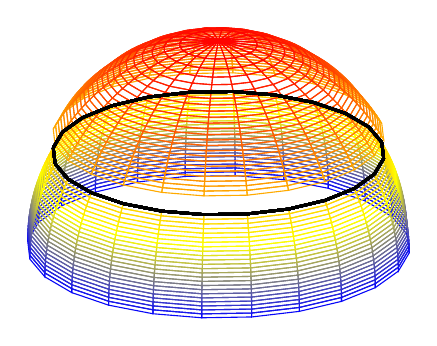
\begin{tikzpicture}
\begin{axis}[
    hide axis,
    view={40}{-30},
    samples=25
]
\addplot3 [
    mesh,
    domain=0:360,
    y domain=0:0.5,
] (
    {cos(x)*sqrt(1-y^2)},
    {sin(x)*sqrt(1-y^2)},
    y
);

\addplot3 [
    mesh,
    domain=0:360,
    y domain=0.5:1,
] (
    {cos(x)*sqrt(1-y^2)},
    {sin(x)*sqrt(1-y^2)},
    y+0.1
);

\addplot3 [
    mesh,
    domain=0:360,
    color=black,
    line width=1pt,
] (
    {cos(x)*sqrt(1-.5^2)},
    {sin(x)*sqrt(1-.5^2)},
    .5
);

% \addplot3 [
%     mesh,
%     color=black,
%     samples=50,
%     domain=0:360,
%     y domain=0:.866,
% ] (
%     {cos(x)*y},
%     {sin(x)*y},
%     0.5
% );

\end{axis}
\end{tikzpicture}

\end{frame}

\begin{frame}
\frametitle{The Breakthrough of Trigonometry}

\begin{center}
We can analyze arbitrary triangles using tools developed for right triangles
\end{center}

\end{frame}

\begin{frame}
\frametitle{The Breakthrough of Calculus}

\begin{center}
We can analyze (most) plane shapes by analyzing shapes with three straight line sides
and a function defining the fourth.
\end{center}

\end{frame}

\begin{frame}
\frametitle{The Breakthrough of Calculus}

\begin{center}
We can vary the position of the right side of this region and get an ``area function''
(an indefinite integral)

We couldn't do this before we restricted our attension to these straight-sided shapes.
\end{center}

\end{frame}

\begin{frame}
\frametitle{The Fundamental Theorem of Calculus}
\end{frame}

\begin{frame}
\frametitle{Berkeley, {\it The Analyst} (1734)}

    And what are these Fluxions? The Velocities of evanescent Increments? And what are these same evanescent Increments? They are neither finite Quantities nor Quantities infinitely small, nor yet nothing. May we not call them the ghosts of departed quantities?[4]

Mathematics historian Judith Grabiner comments, "Berkeley's criticisms of the rigor of the calculus were witty, unkind, and — with respect to the mathematical practices he was criticizing — essentially correct".[8] While his critiques of the mathematical practices were sound, his essay has been criticized on logical and philosophical grounds. 

Source: Wikipedia, {\it The Analyst}
\end{frame}

\begin{frame}
\frametitle{Slope of a Parabola}
\end{frame}

\begin{frame}
\frametitle{Augustin-Louis Cauchy, {\it Cours D'Analyse} (1821)}

Limits

Derivative (definition)

Continuity (definition)

Theorem: Polynomials are continuous everywhere

Use limits and the theorem to compute derivative of a parabola
\end{frame}

\begin{frame}
\frametitle{Bernhard Riemann - The Riemann Integral}
\end{frame}

\begin{frame}
\frametitle{Georg Cantor - Set Theory}

Two sets are of equal size (cardinality) if a one-to-one mapping can be set up between them.

Rational numbers have the same cardinality as the integers

Integers, rationals, tuples of integers and rationals all have the same cardinality

They are ``countable''

The real numbers are {\it not} countable.

Their cardinality in the ``continuum''
\end{frame}

\begin{frame}
\frametitle{Henri Lebesgue - ``Integral, Length, Area'' (1902)}


\end{frame}

\end{document}
